\documentclass[11pt,xcolor=table]{beamer}
\usetheme[
%%% options passed to the outer theme
 %   hidetitle,           % hide the (short) title in the sidebar
    hideauthor,          % hide the (short) author in the sidebar
%    hideinstitute,       % hide the (short) institute in the bottom of the sidebar
%    shownavsym,          % show the navigation symbols
%    width=2cm,           % width of the sidebar (default is 2 cm)
%    hideothersubsections,% hide all subsections but the subsections in the current section
%    hideallsubsections,  % hide all subsections
    left               % right of left position of sidebar (default is right)
%%% options passed to the color theme
%    lightheaderbg,       % use a light header background
  ]{AAUsidebar}
\setbeamertemplate
    {frametitle}
    {
      \begin{flushright}
        \insertframetitle
      \end{flushright}
    }
\mode<presentation>
{
  \setbeamertemplate{navigation symbols}{}
  \setbeamertemplate{caption}[numbered]
  \setbeamertemplate{itemize subitem}[triangle]
 % \setbeameroption{show notes}
} 


% If you want to change the colors of the various elements in the theme, edit and uncomment the following lines
% Change the bar and sidebar colors:
%\setbeamercolor{AAUsidebar}{fg=gray!50,bg=gray}
%\setbeamercolor{sidebar}{bg=red!20}
% Change the color of the structural elements:
%\setbeamercolor{structure}{fg=red}
% Change the frame title text color:
%\setbeamercolor{frametitle}{fg=blue}
% Change the normal text color background:
%\setbeamercolor{normal text}{bg=gray!10}
% ... and you can of course change a lot more - see the beamer user manual.

\usepackage{tikz}   

\usepackage[utf8]{inputenc}
\usepackage[english]{babel}
\usepackage[T1]{fontenc}
\usepackage{helvet}
\usepackage{array}
\newcolumntype{L}[1]{>{\raggedright\let\newline\\\arraybackslash\hspace{0pt}}m{#1}}
\newcolumntype{C}[1]{>{\centering\let\newline\\\arraybackslash\hspace{0pt}}m{#1}}
\newcolumntype{R}[1]{>{\raggedleft\let\newline\\\arraybackslash\hspace{0pt}}m{#1}}
\usepackage{multirow}
\definecolor{Gray}{gray}{0.9}
% colored hyperlinks
\newcommand{\chref}[2]{%
  \href{#1}{{\usebeamercolor[bg]{AAUsidebar}#2}}%
}

\title[Sequencing, Statistical Genetics and HLA\\11/10/2015]% optional, use only with long paper titles
{Dissecting Peruvian population structure based on 1000 Genomes Phase 3 dataset}
%\vspace{5cm}
%\subtitle{TBRU progress report}  % could also be a conference name

\date{November 10, 2015}

\author[Yang Luo] % optional, use only with lots of authors
{
  Yang Luo \\
  \vskip2pt
  \href{mailto:yangluo@broadinstitute.org}{{\tt yangluo@broadinstitute.org }}
}
% - Give the names in the same order as they appear in the paper.
% - Use the \inst{?} command only if the authors have different
%   affiliation. See the beamer manual for an example

\institute[Raychaudhuri's Lab] 
{% is placed on the title page
 % \small{Human Genetics, Wellcome Trust Sanger Institute, UK}
  
  %there must be an empty line above this line - otherwise some unwanted space is added between the university and the country (I do not know why;( )
}


% specify a logo on the titlepage (you can specify additional logos an include them in 
% institute command below
%\pgfdeclareimage[height=1.8cm]{titlepagelogo}{pics/sang_logo_large.png} % placed on the title page
%\pgfdeclareimage[height=1.5cm]{titlepagelogo2}{graphics/aau_logo_new} % placed on the title page
%\titlegraphic{% is placed on the bottom of the title page
%  \pgfuseimage{titlepagelogo}
%  \hspace{1cm}\pgfuseimage{titlepagelogo2}
%}

\AtBeginSection{\frame{\sectionpage}}

\begin{document}
% the titlepage
{\aauwavesbg%
\begin{frame}[plain,noframenumbering] % the plain option removes the sidebar and header from the title page
  \titlepage
\end{frame}}
%%%%%%%%%%%%%%%%

% TOC
%\begin{frame}{Outlines}{}
%\tableofcontents
%\end{frame}
%%%%%%%%%%%%%%%%

\section[1000Genomes]{Dissecting Peruvian population structure based on 1000 Genomes Phase 3 dataset}
% motivation for creating this theme
\subsection{Data description}
\begin{frame}{What's in 1000 genomes phase 3?}
\begin{block}{26 different populations from  different locations around the globe.}
\end{block}
\begin{table}[1000 Genomes Samples]
\centering
\begin{tabular}{|r|r|}
\hline
 {\bf Population}& {\bf Size}  \\ \hline\hline
East Asian Ancestry (EAS)& 504 \\\hline
South Asian Ancestry (SAS)& 489 \\ \hline
African Ancestry (AFR) &661\\\hline
 European Ancestry (EUR) & 503 \\\hline
 \bf{Americas Ancestry (AMR)} & \bf 347 \\\hline
 Total &2504\\\hline
\end{tabular}
\end{table}

\end{frame}
\begin{frame}{What's included in AMR?}
\begin{block}{Four populations with Americas ancestry}
\end{block}
\begin{table}[]
\centering
\small
\begin{tabular}{|r|r|}
\hline
\bf Population & \bf Size \\ \hline
Colombian in Medellin, Colombia (CLM) & 94 \\ \hline
Mexican Ancestry in Los Angeles, California (MXL) & 64 \\ \hline
\bf Peruvian in Lima, Peru (PEL) & \bf 85 \\ \hline
Puerto Rican in Puerto Rico (PUR) & 104 \\ \hline
Total & 347 \\ \hline
\end{tabular}
\end{table}

\end{frame}

\begin{frame}{Data origins}
\centering
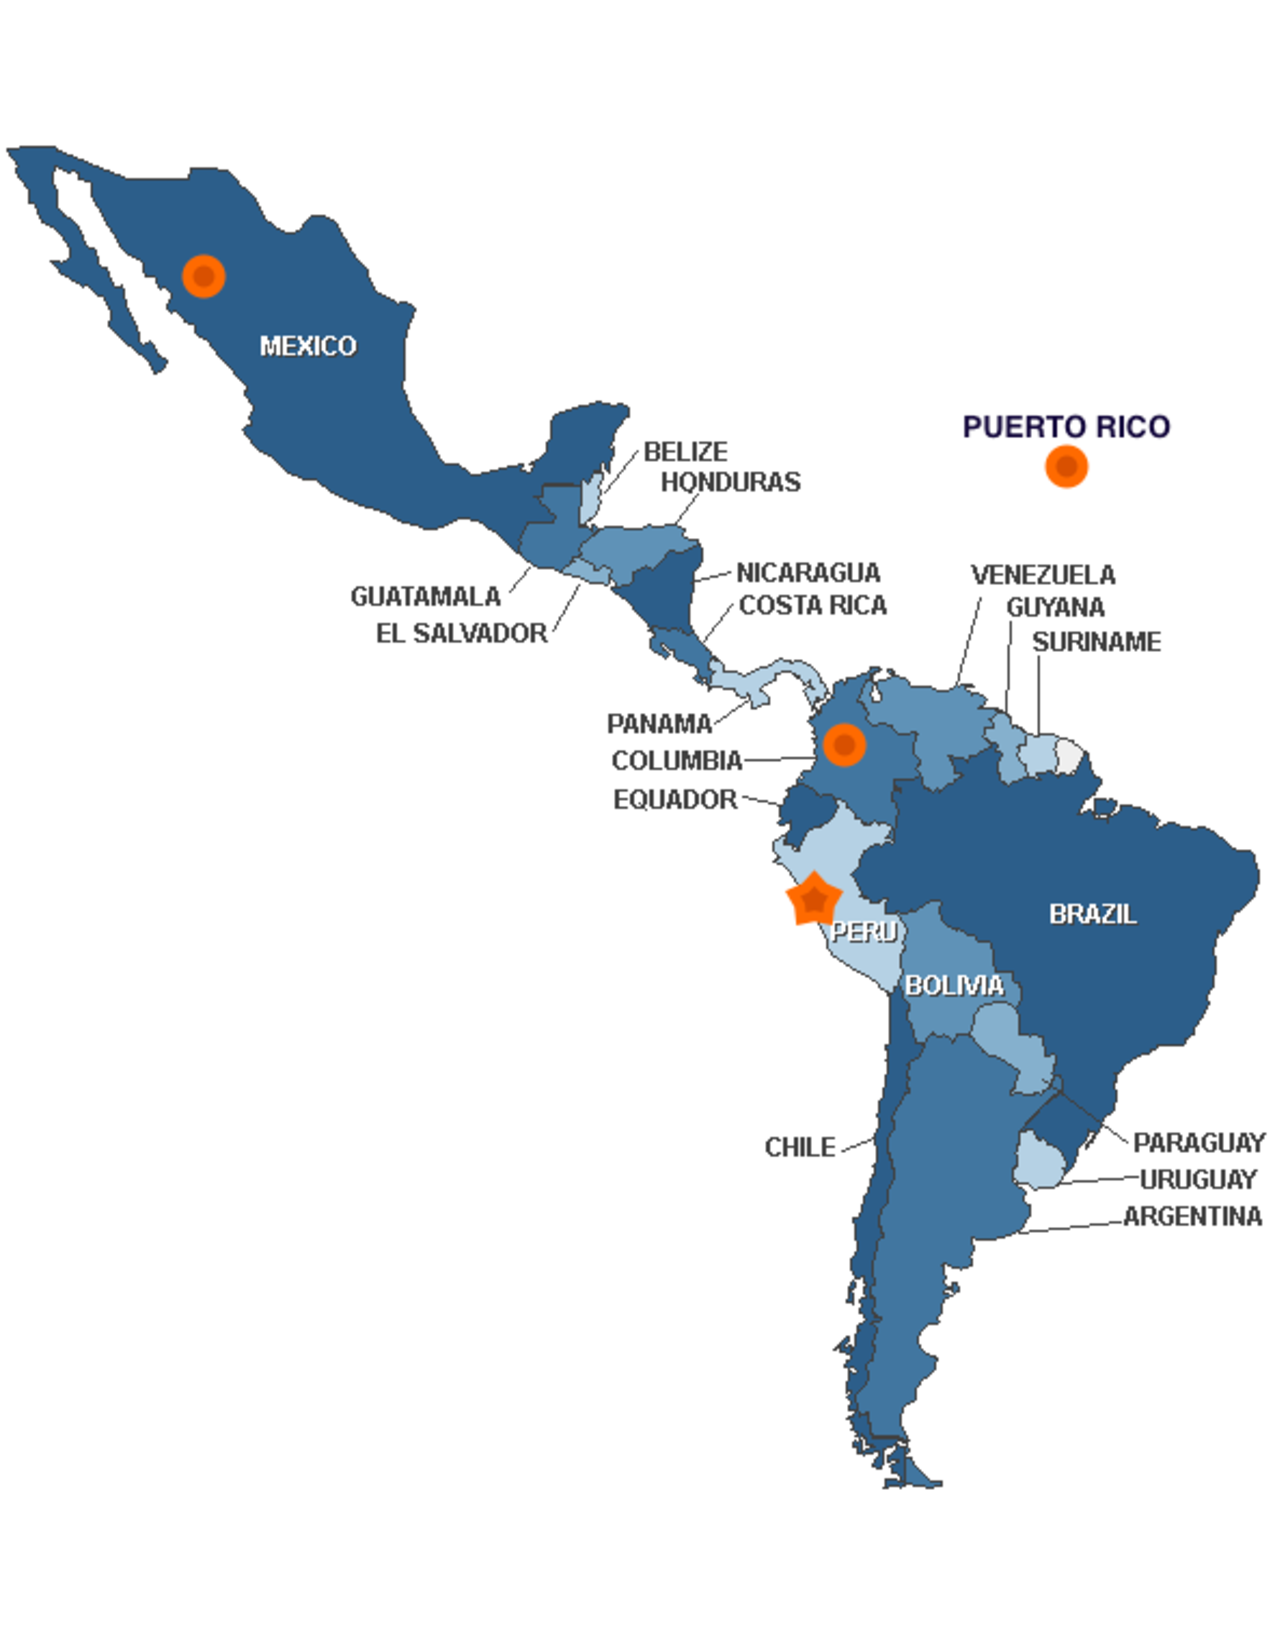
\includegraphics[width=.8\textwidth]{pics/south_america_map.pdf}
\end{frame}

\subsection{Population Structure in Peruvian}
\begin{frame}{Questions we are interested in asking}
\begin{block}{How different is the Peruvian population vs those of other populations?}
\only<2>{
\begin{itemize}
\item Principal component analysis
\item $F_{st}$ estimate
\item How many variants are unique to Peruvians
\end{itemize}}
\end{block}
\begin{block}{Where does the current Peruvian population originate from?}
\only<2>{Ancestry inference: ADMIXTURE analysis}
\end{block}

\end{frame}
\subsubsection{Principal component analysis}
\begin{frame}{1000 Genomes Phase 3 Population PCs}
\only<1>{
\centering
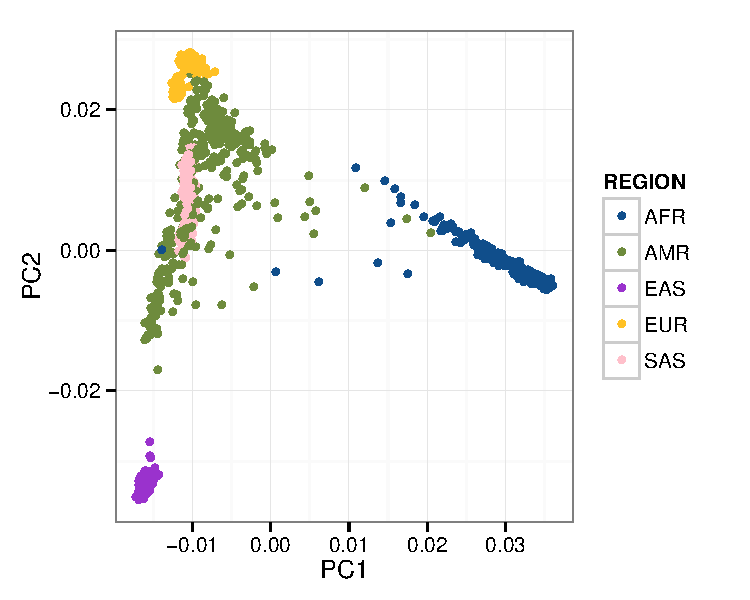
\includegraphics[width=1\textwidth]{pics/G1K-REGION-PCs.pdf}
}
\only<2>{
\centering
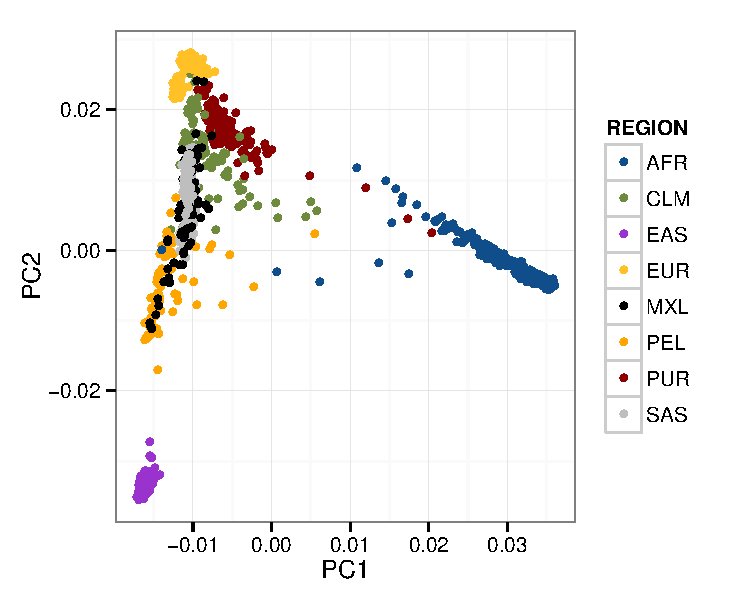
\includegraphics[width=1\textwidth]{pics/G1K-AMR-others-PCs.pdf}
}
\end{frame}

\begin{frame}{Peruvian PCs}
\centering
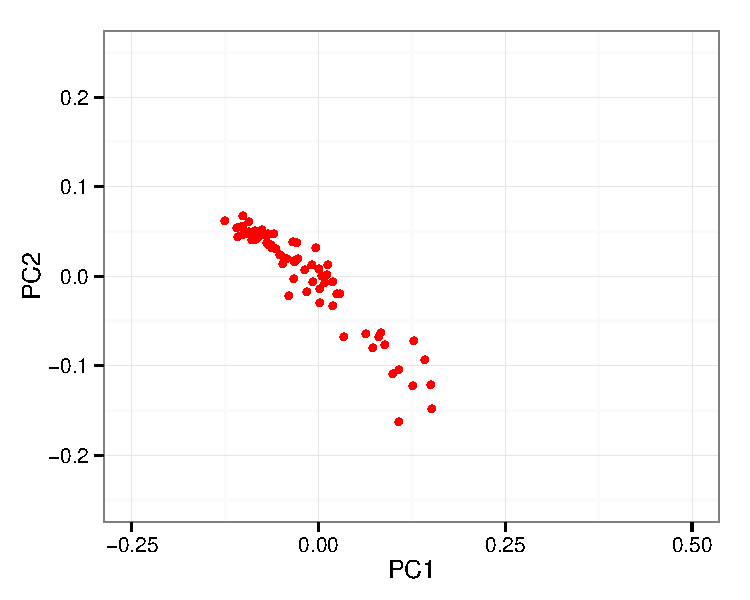
\includegraphics[width=1\textwidth]{pics/pel.pdf}
\end{frame}

\begin{frame}{\scriptsize{East Asian -- Chinese Dai; Beijing; Southern Chinese; Tokyo; Ho Chi Minh City}}
\centering
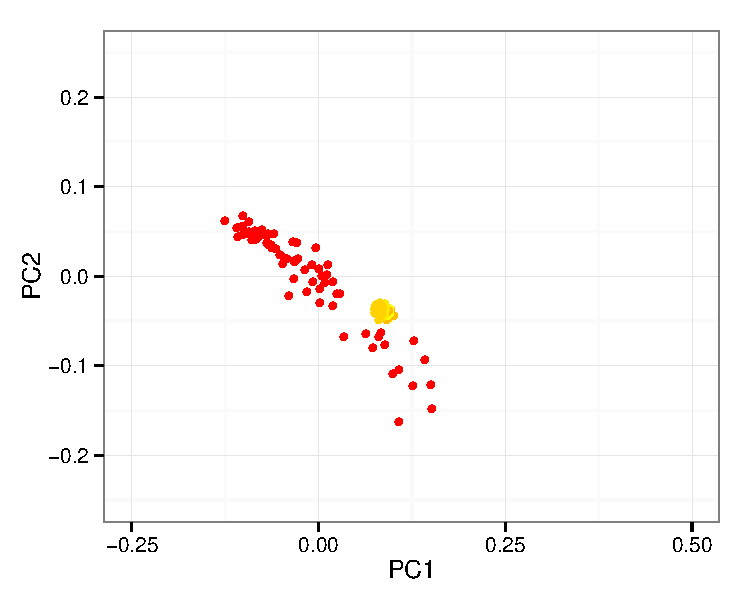
\includegraphics[width=1\textwidth]{pics/pel-EAS.pdf}
\end{frame}

\begin{frame}{\scriptsize{South Asian -- Bangladesh; Gujarati Indian in Houston;\\ Indian Telugu in UK; Punjabi in Lahore; Sri Lankan Tamil}}
\centering
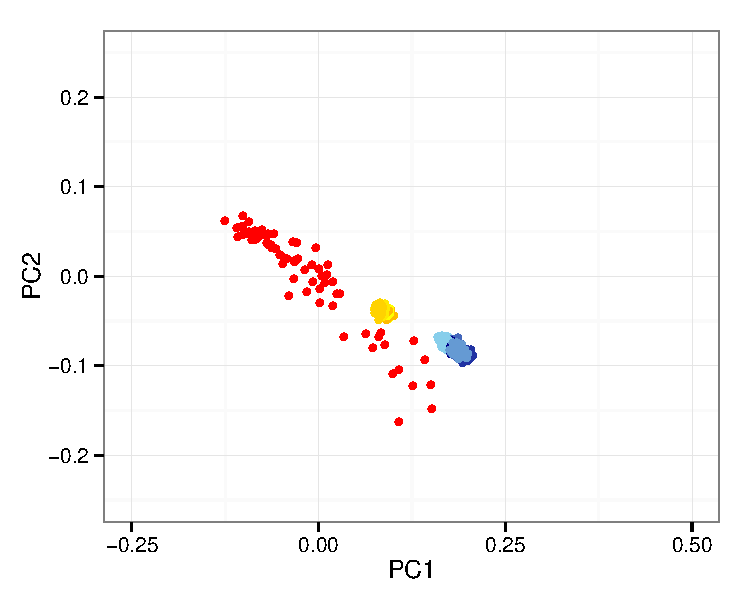
\includegraphics[width=1\textwidth]{pics/pel-EAS-SAS.pdf}
\end{frame}

\begin{frame}{\scriptsize{African -- African in Southwest US; African Caribbean; Esan; Gambian; Luhya; \\Sierra Leone; Yoruba in Ibadan}}
\centering
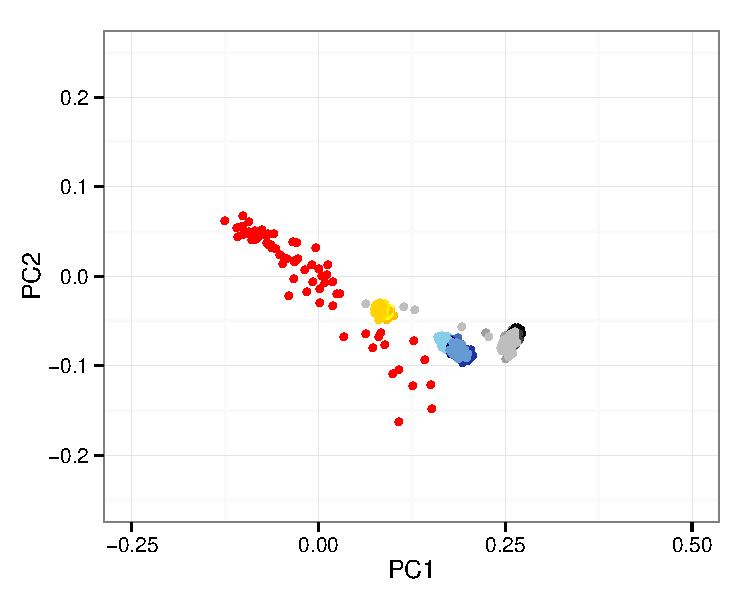
\includegraphics[width=1\textwidth]{pics/pel-EAS-SAS-AFR.pdf}
\end{frame}

\begin{frame}{\scriptsize{European -- British; Finnish; Iberian; Toscani; Utah residents with Northern\\ and Western European ancestry }}
\centering
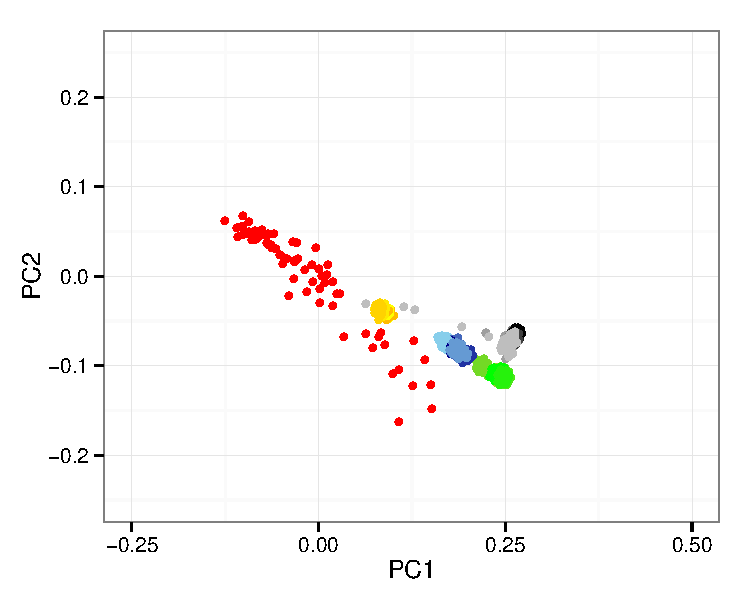
\includegraphics[width=1\textwidth]{pics/pel-EUR.pdf}
\end{frame}

\begin{frame}{All- 26 populations}
\centering
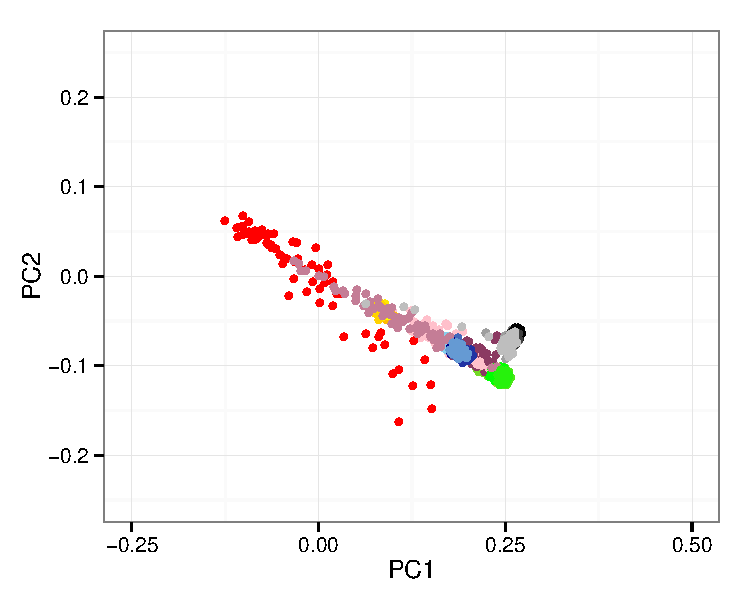
\includegraphics[width=1\textwidth]{pics/pel-ALL.pdf}
\end{frame}

\begin{frame}{Americas}
\centering
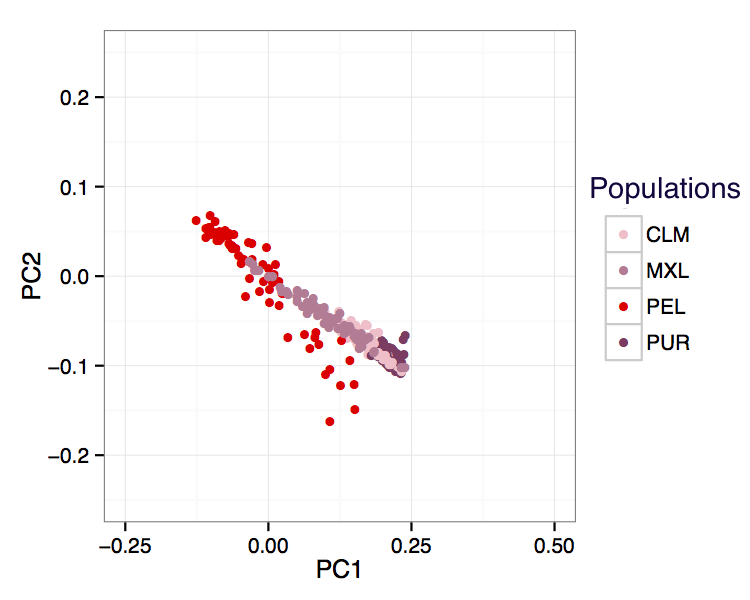
\includegraphics[width=.85\textwidth]{pics/pel-AMR.png}
\end{frame}

\subsubsection{Fst estimation}
\begin{frame}{Fst*1000 in Americas}
\begin{block}{A measure of population differentiation due to genetic structure}
\end{block}
\begin{table}[]
\centering
\begin{tabular}{|r||r|r|r|r|}
\hline
    &PUR    &    CLM    &    PEL&        MXL \\ \hline
PUR&      0   &  6    &61  &  20 \\ \hline
CLM &     6  &   0    &42  &  10 \\ \hline
PEL  &   61 &   42    & 0 &   18 \\ \hline
MXL   &  20&    10    &18&     0 \\ \hline
\end{tabular}
\end{table}
\end{frame}

\subsubsection{Private variants}
\begin{frame}{Variants that are unique to Peruvians}
\centering
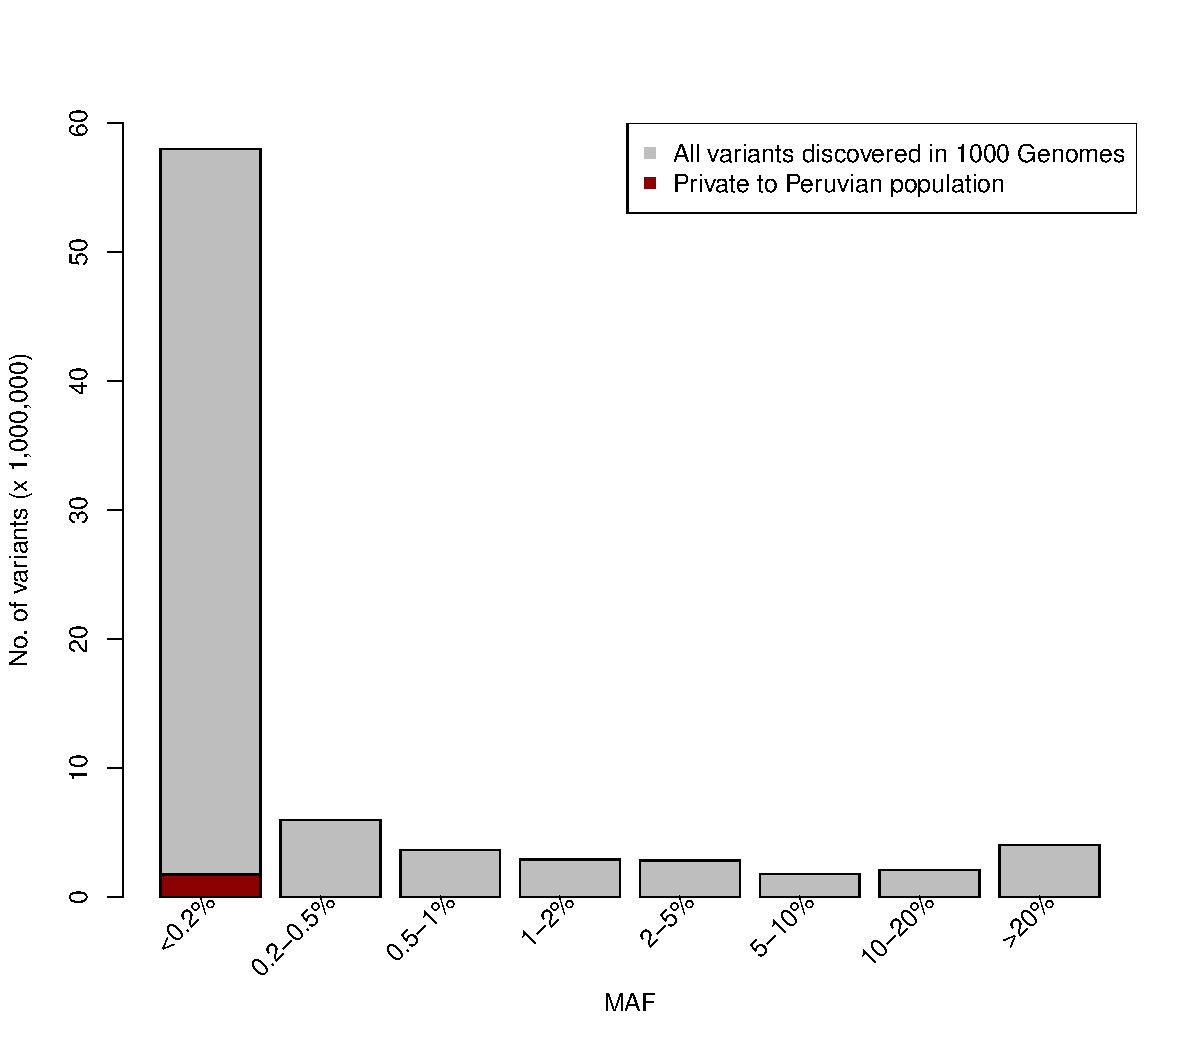
\includegraphics[width=1\textwidth]{pics/all-frq-private-pel.pdf}
\end{frame}
\begin{frame}{Frequencies of these private variants}
\centering
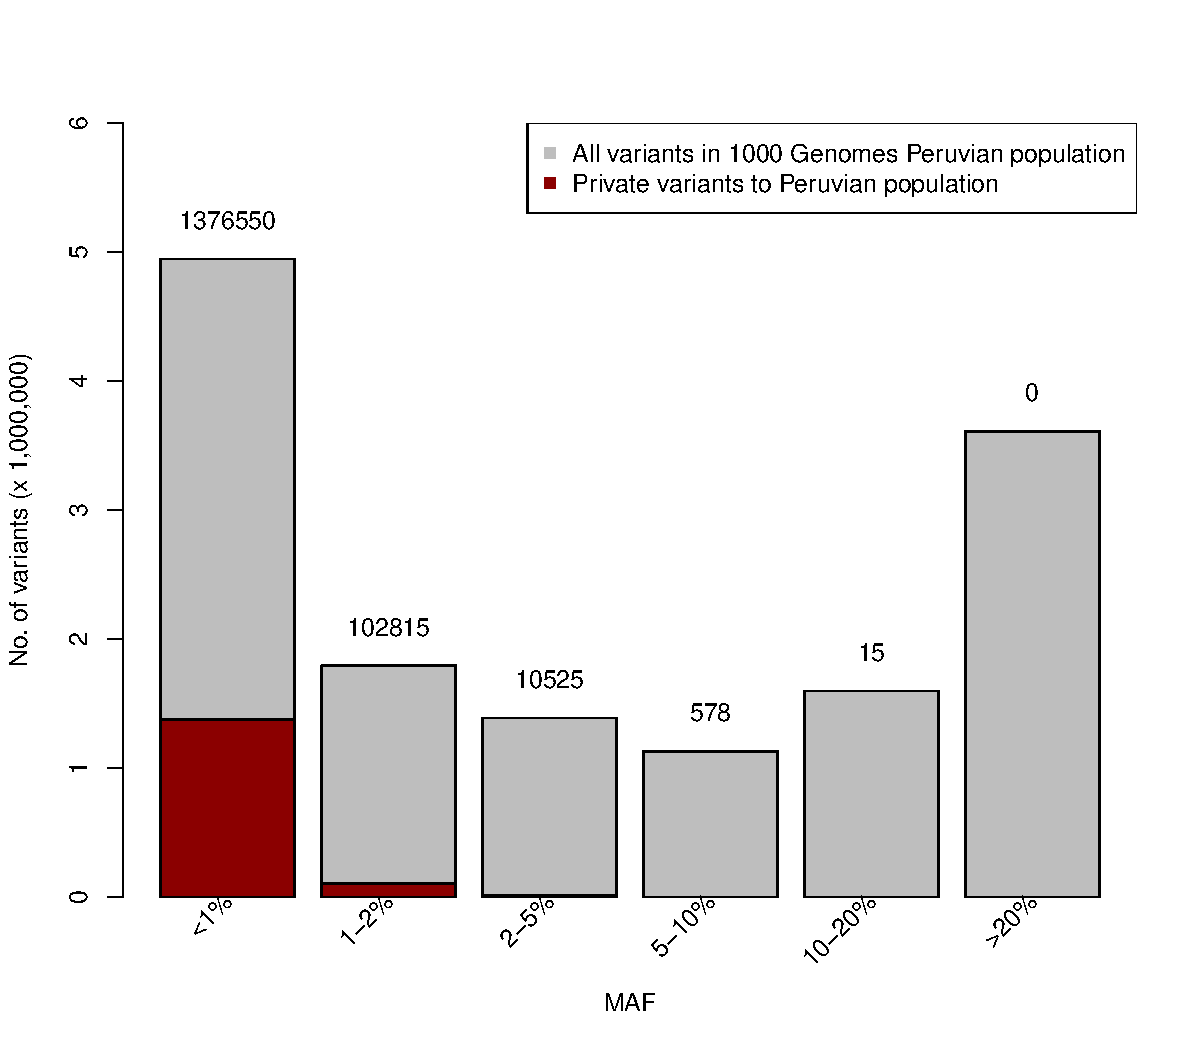
\includegraphics[width=1\textwidth]{pics/pel-frq-private-pel.pdf}
\end{frame}

\subsubsection{Ancestral clusters}
\begin{frame}{ADMIXTURE analysis}
\centering
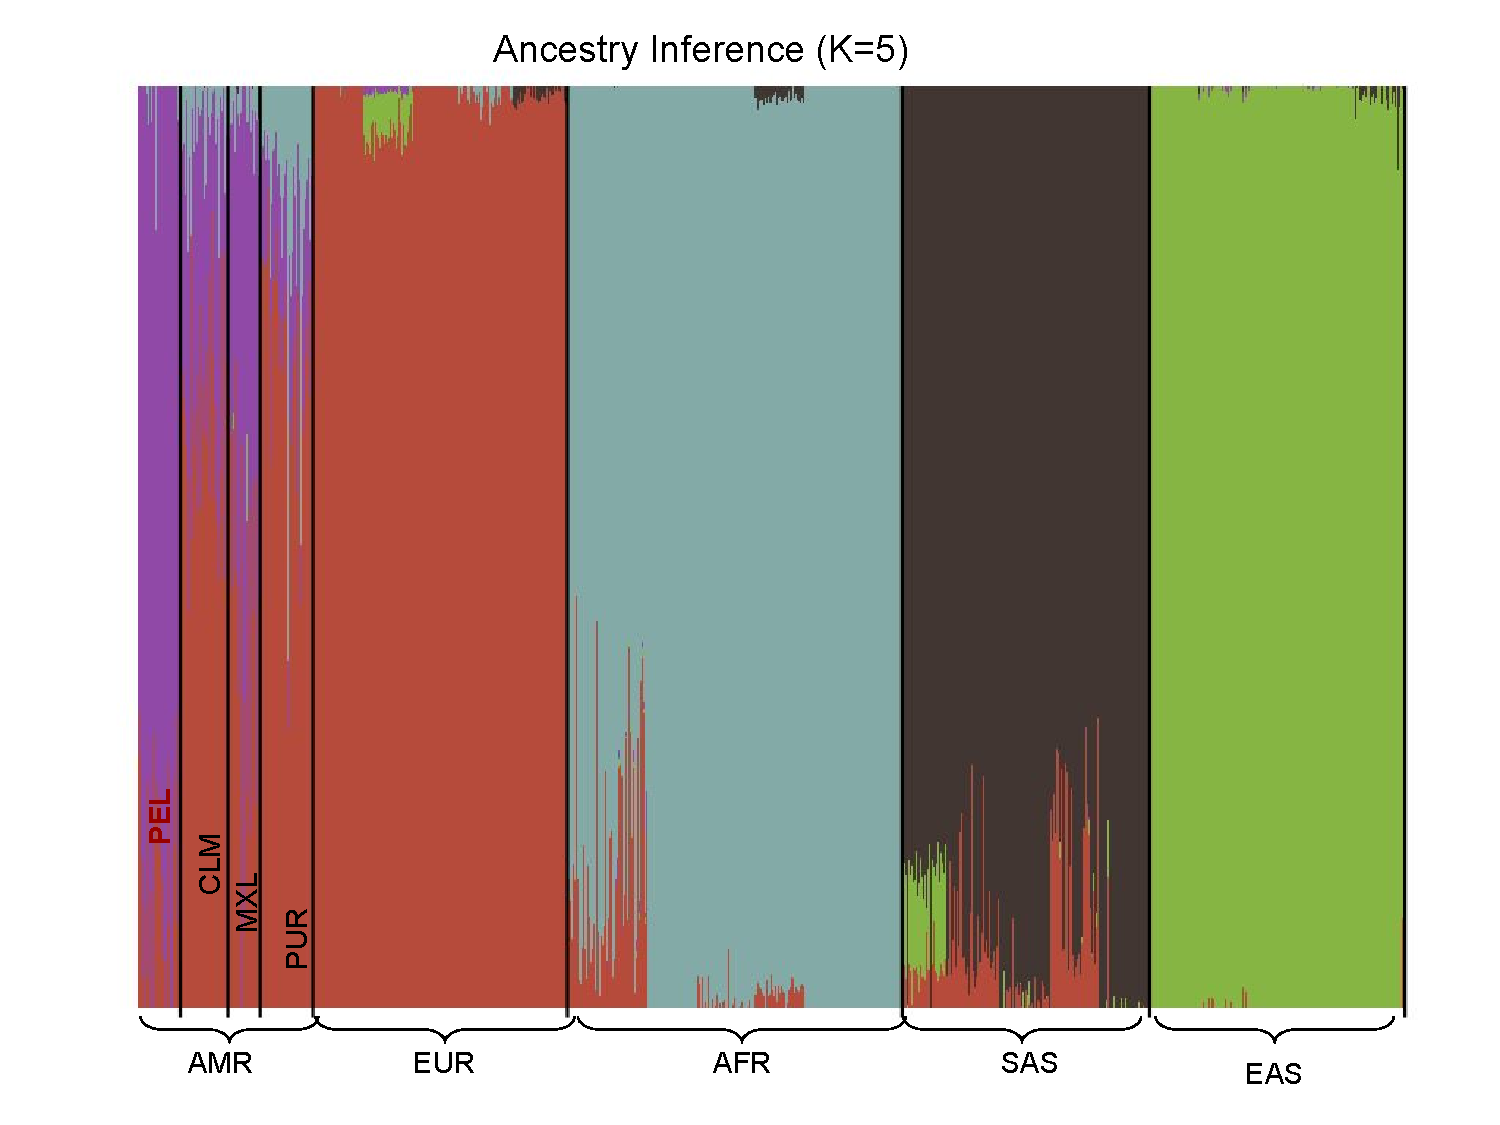
\includegraphics[width=1.05\textwidth]{pics/g1k_admixture.pdf}
\end{frame}

\begin{frame}{Add some more data -- HGDP}
\begin{table}[]
\centering
\begin{tabular}{|r|r|}
\hline
Super Population & no. of samples \\
\hline
North Africa  & 29 \\
Subsaharian Africa & 105 \\
{\bf{America}} & \bf 64  \\
Asia    &434 \\
Middle Est     &134 \\
Europe  &158 \\
Oceania &28 \\
\hline
\end{tabular}
\end{table}
\begin{itemize}
\item 940 samples in total
\item 6 super populations
\item 57 sub populations, of which 5 are from America:
\begin{itemize}
\item Colombians (Columbia)      7
\item Karitiana (Brazil)      14
\item Maya (Mexico)  21
\item Pima (Mexico)   14
\item Surui (Brazil)   8
\end{itemize}
\end{itemize}
\end{frame}
\begin{frame}{Ancestral clusters including HGDP data}
\centering
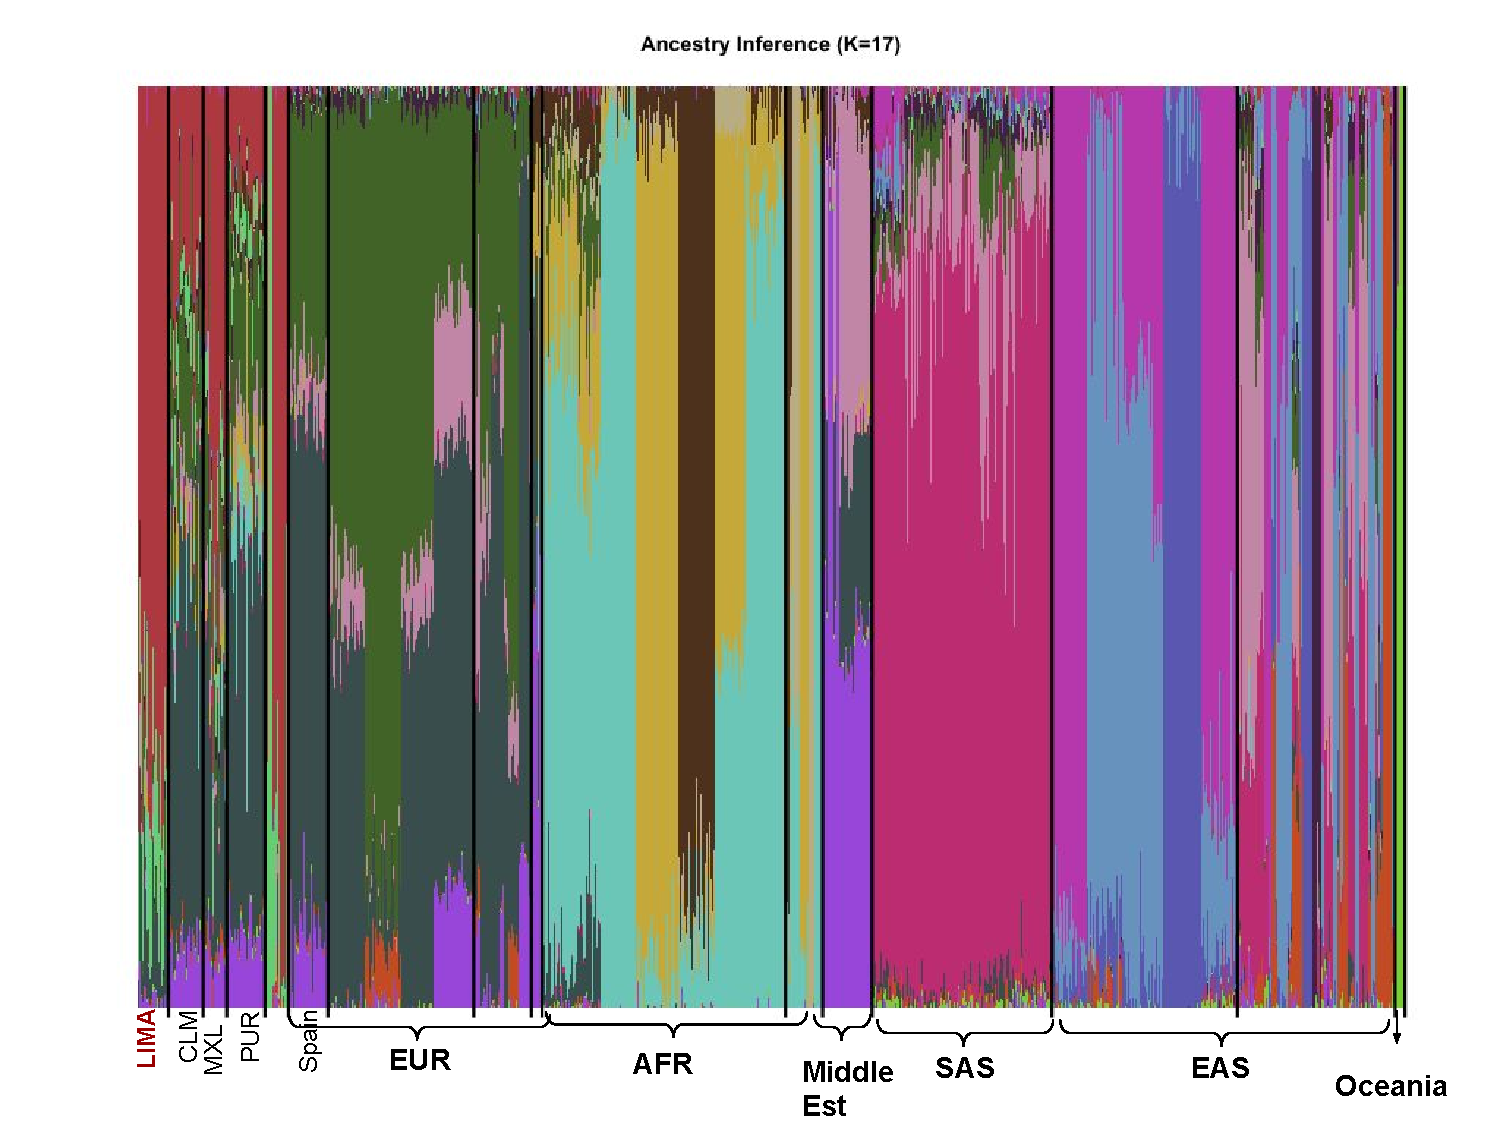
\includegraphics[width=1.05\textwidth]{pics/admixture_plot.pdf}
\end{frame}

\begin{frame}{Nonrandom mating?}
\centering

\includegraphics[width=1\textwidth]{pics/Zou_et_al.png}
\end{frame}

\section{Reproducible research}
\begin{frame}{Aims}
\begin{itemize}
\item Reproducing my own results 
\item Making small modifications -- change input files; scale it up
\item Easier for others to use -- carry on or similar tasks
\item Usable for everyone -- code release
\end{itemize}
\end{frame}
\begin{frame}{Methods}
\begin{itemize}
\item Simple Bash \href{https://github.com/yluo86/LIMAA/blob/master/sandbox/scripts/1kg_process.sh}{\beamergotobutton{Bash script}}
\item Bpipe \href{https://github.com/yluo86/LIMAA/blob/master/sandbox/scripts/1kg_process.pipebpipe}{\beamergotobutton{bpipe}}
\item Snakemake?
\end{itemize}
\end{frame}


\section{Choosing controls}
\subsection{Motivation}
\begin{frame}{Study design for GWAS}
\begin{block}{Problem}
We have 1500 active TB cases. Under the same household, do we choose unrelated controls or 1st degree relatives?
\end{block}
\begin{block}{Approach}
Simulate a number of genotype data (related or unrelated) and risk alleles with different ORs. Empirically calculates the discover rate of the risk alleles.
\end{block}
\end{frame}

\subsection{Simulations}
\begin{frame}{Power to discover $1\%$ variants}
\centering
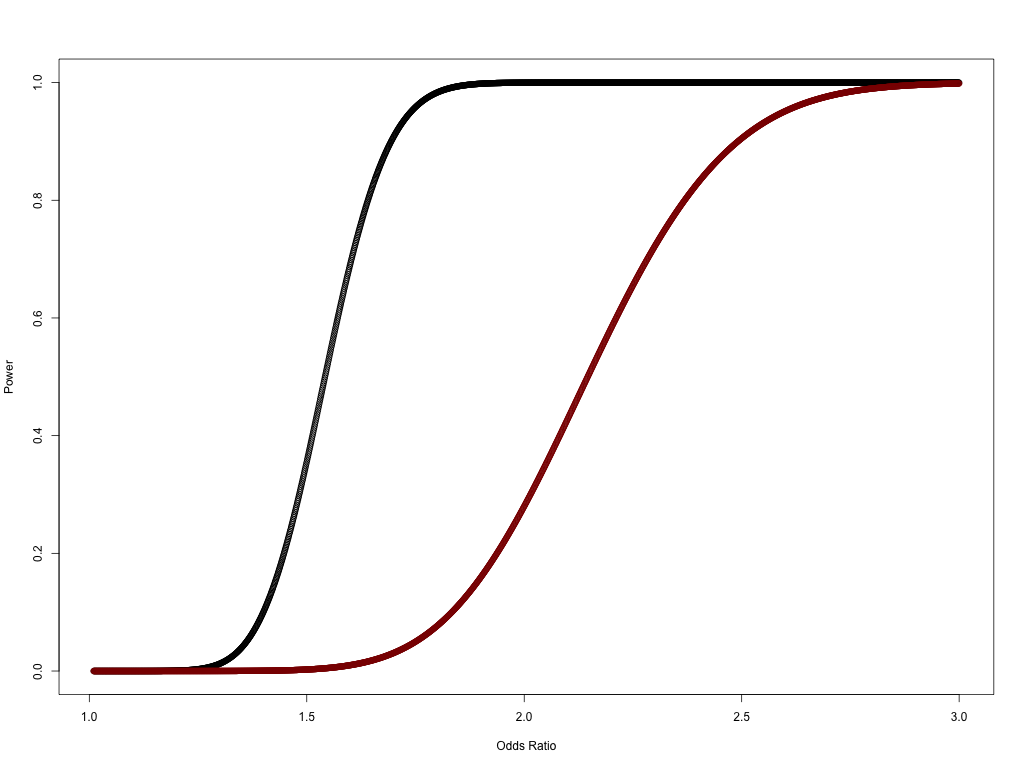
\includegraphics[width=1\textwidth]{pics/power-curve.png}
\end{frame}


\end{document}